

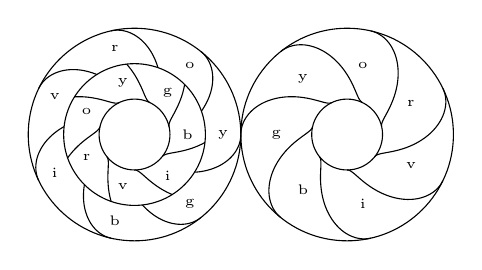
\begin{tikzpicture}[scale=0.45,every node/.style={font=\tiny}]

\def\fo{1/14}
        \begin{scope}[shift={(3,0)}]
        \draw (1,0) arc (0:360:1);
        \draw (3,0) arc (0:360:3);
        \draw[variable=\t,domain=0:0.5,samples=40] plot ({(2+cos(\t*360))*cos(\t*360*5*\fo+7*\fo*360+0*\fo*360)},{(2+cos(\t*360))*sin(\t*360*5*\fo+0*\fo*360)});
        \draw[variable=\t,domain=0:0.5,samples=40] plot ({(2+cos(\t*360))*cos(\t*360*5*\fo+7*\fo*360+2*\fo*360)},{(2+cos(\t*360))*sin(\t*360*5*\fo+2*\fo*360)});
        \draw[variable=\t,domain=0:0.5,samples=40] plot ({(2+cos(\t*360))*cos(\t*360*5*\fo+7*\fo*360+4*\fo*360)},{(2+cos(\t*360))*sin(\t*360*5*\fo+4*\fo*360)});
        \draw[variable=\t,domain=0:0.5,samples=40] plot ({(2+cos(\t*360))*cos(\t*360*5*\fo+7*\fo*360+6*\fo*360)},{(2+cos(\t*360))*sin(\t*360*5*\fo+6*\fo*360)});
        \draw[variable=\t,domain=0:0.5,samples=40] plot ({(2+cos(\t*360))*cos(\t*360*5*\fo+7*\fo*360+8*\fo*360)},{(2+cos(\t*360))*sin(\t*360*5*\fo+8*\fo*360)});
        \draw[variable=\t,domain=0:0.5,samples=40] plot ({(2+cos(\t*360))*cos(\t*360*5*\fo+7*\fo*360+10*\fo*360)},{(2+cos(\t*360))*sin(\t*360*5*\fo+10*\fo*360)});
        \draw[variable=\t,domain=0:0.5,samples=40] plot ({(2+cos(\t*360))*cos(\t*360*5*\fo+7*\fo*360+12*\fo*360)},{(2+cos(\t*360))*sin(\t*360*5*\fo+12*\fo*360)});
        \node at (180-0*\fo*360:2){g};
        \node at (180-2*\fo*360:2){y};
        \node at (180-4*\fo*360:2){o};
        \node at (180-6*\fo*360:2){r};
        \node at (180+2*\fo*360:2){b};
        \node at (180+4*\fo*360:2){i};
        \node at (180+6*\fo*360:2){v};
        \end{scope}
        \begin{scope}[shift={(-3,0)}]
        \draw (1,0) arc (0:360:1);
        \draw (2,0) arc (0:360:2);
        \draw (3,0) arc (0:360:3);
        \draw[variable=\t,domain=-0.25:0,samples=40] plot ({(2+cos(\t*360))*cos(\t*360*5*\fo+0*\fo*360)},{(2+cos(\t*360))*sin(\t*360*5*\fo+0*\fo*360)});
        \draw[variable=\t,domain=0.5:0.75,samples=40] plot ({(2+cos(\t*360))*cos(\t*360*5*\fo+0*\fo*360)},{(2+cos(\t*360))*sin(\t*360*5*\fo+0*\fo*360)});
        \draw[variable=\t,domain=-0.25:0,samples=40] plot ({(2+cos(\t*360))*cos(\t*360*5*\fo+2*\fo*360)},{(2+cos(\t*360))*sin(\t*360*5*\fo+2*\fo*360)});
        \draw[variable=\t,domain=0.5:0.75,samples=40] plot ({(2+cos(\t*360))*cos(\t*360*5*\fo+2*\fo*360)},{(2+cos(\t*360))*sin(\t*360*5*\fo+2*\fo*360)});
        \draw[variable=\t,domain=-0.25:0,samples=40] plot ({(2+cos(\t*360))*cos(\t*360*5*\fo+4*\fo*360)},{(2+cos(\t*360))*sin(\t*360*5*\fo+4*\fo*360)});
        \draw[variable=\t,domain=0.5:0.75,samples=40] plot ({(2+cos(\t*360))*cos(\t*360*5*\fo+4*\fo*360)},{(2+cos(\t*360))*sin(\t*360*5*\fo+4*\fo*360)});
        \draw[variable=\t,domain=-0.25:0,samples=40] plot ({(2+cos(\t*360))*cos(\t*360*5*\fo+6*\fo*360)},{(2+cos(\t*360))*sin(\t*360*5*\fo+6*\fo*360)});
        \draw[variable=\t,domain=0.5:0.75,samples=40] plot ({(2+cos(\t*360))*cos(\t*360*5*\fo+6*\fo*360)},{(2+cos(\t*360))*sin(\t*360*5*\fo+6*\fo*360)});
        \draw[variable=\t,domain=-0.25:0,samples=40] plot ({(2+cos(\t*360))*cos(\t*360*5*\fo+8*\fo*360)},{(2+cos(\t*360))*sin(\t*360*5*\fo+8*\fo*360)});
        \draw[variable=\t,domain=0.5:0.75,samples=40] plot ({(2+cos(\t*360))*cos(\t*360*5*\fo+8*\fo*360)},{(2+cos(\t*360))*sin(\t*360*5*\fo+8*\fo*360)});
        \draw[variable=\t,domain=-0.25:0,samples=40] plot ({(2+cos(\t*360))*cos(\t*360*5*\fo+10*\fo*360)},{(2+cos(\t*360))*sin(\t*360*5*\fo+10*\fo*360)});
        \draw[variable=\t,domain=0.5:0.75,samples=40] plot ({(2+cos(\t*360))*cos(\t*360*5*\fo+10*\fo*360)},{(2+cos(\t*360))*sin(\t*360*5*\fo+10*\fo*360)});
        \draw[variable=\t,domain=-0.25:0,samples=40] plot ({(2+cos(\t*360))*cos(\t*360*5*\fo+12*\fo*360)},{(2+cos(\t*360))*sin(\t*360*5*\fo+12*\fo*360)});
        \draw[variable=\t,domain=0.5:0.75,samples=40] plot ({(2+cos(\t*360))*cos(\t*360*5*\fo+12*\fo*360)},{(2+cos(\t*360))*sin(\t*360*5*\fo+12*\fo*360)});
        \node at (0*\fo*360:1.5){b};
        \node at (2*\fo*360:1.5){g};
        \node at (4*\fo*360:1.5){y};
        \node at (6*\fo*360:1.5){o};
        \node at (8*\fo*360:1.5){r};
        \node at (10*\fo*360:1.5){v};
        \node at (12*\fo*360:1.5){i};
        \node at (0*\fo*360:2.5){y};
        \node at (2*\fo*360:2.5){o};
        \node at (4*\fo*360:2.5){r};
        \node at (6*\fo*360:2.5){v};
        \node at (8*\fo*360:2.5){i};
        \node at (10*\fo*360:2.5){b};
        \node at (12*\fo*360:2.5){g};
        \end{scope}
\end{tikzpicture}